\documentclass[a4paper]{article}
\usepackage{graphicx}
\usepackage{amsmath,amssymb}
\usepackage{hyperref}

\title{Meta cognition}
\date{}
\begin{document}
    \maketitle
    Metacognition is an awareness of one's thought processes and an understanding of the patterns behind them.
    \url{https://en.wikipedia.org/wiki/Metacognition}
    
    Also this book for a neuro science perspective
    \url{https://link.springer.com/book/10.1007/978-3-642-45190-4}
    \\
    \url{https://www.amazon.de/-/en/Cognitive-Neuroscience-Metacognition-Stephen-Fleming/dp/3662511711}
    \paragraph{Image}
    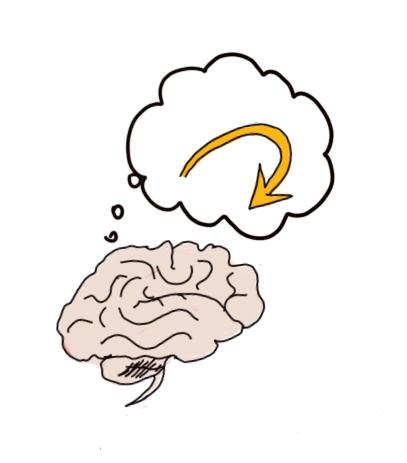
\includegraphics[scale=1]{meta.png}
    
    
    \section{Metacognitive Knowledge}
    \begin{itemize}
        \item \textbf{Definition:} Knowledge that a system has about its own cognitive processes, such as what it knows, what it does not know, and how it learns.
        \item \textbf{Typical components:}
        \begin{itemize}
            \item Knowledge of knowledge states
            \item Knowledge of strategies
            \item Knowledge of task difficulty
        \end{itemize}
    \end{itemize}
    
    
    \section{Metacognitive Monitoring}
    \begin{itemize}
        \item \textbf{Definition:} The process by which a system observes and evaluates its ongoing cognitive activities.
        \item \textbf{Typical functions:}
        \begin{itemize}
            \item Error detection
            \item Confidence estimation
            \item Uncertainty estimation
        \end{itemize}
    \end{itemize}
    
    
    \section{Metacognitive Control}
    \begin{itemize}
        \item \textbf{Definition:} The ability of a system to regulate or adjust its cognitive processes based on monitoring results.
        \item \textbf{Typical actions:}
        \begin{itemize}
            \item Changing strategies
            \item Allocating attention
            \item Requesting more information
        \end{itemize}
    \end{itemize}
    
    
    \section{Self-Awareness}
    \begin{itemize}
        \item \textbf{Definition:} The ability of a system to represent and recognize its own internal states and identity.
        \item \textbf{Typical aspects:}
        \begin{itemize}
            \item Self-model
            \item Body awareness
            \item Internal state awareness
        \end{itemize}
    \end{itemize}
    
    
    \section{Meta-Learning}
    \begin{itemize}
        \item \textbf{Definition:} The ability of a system to improve its own learning process through experience.
        \item \textbf{Typical aspects:}
        \begin{itemize}
            \item Learning to learn
            \item Adaptation of learning strategies
            \item Adjustment of learning parameters
        \end{itemize}
    \end{itemize}
    
    
    \section{Introspection}
    \begin{itemize}
        \item \textbf{Definition:} The capacity of a system to internally examine its own reasoning or cognitive states.
        \item \textbf{Typical aspects:}
        \begin{itemize}
            \item Examination of reasoning steps
            \item Evaluation of internal beliefs
            \item Reflection on cognitive states
        \end{itemize}
    \end{itemize}
    
    
    \section{Uncertainty Awareness}
    \begin{itemize}
        \item \textbf{Definition:} The ability of a system to estimate the reliability or uncertainty of its own predictions or decisions.
        \item \textbf{Typical aspects:}
        \begin{itemize}
            \item Confidence estimation
            \item Uncertainty estimation
            \item Reliability assessment of predictions
        \end{itemize}
    \end{itemize}
    
    \paragraph{Examples}
        I know that I don't know
    
        
\end{document}